\chapter{Implementation}
\label{chap:ch4_abbr}
\label{chap:figtab}
\section{Review}
The software implementation showcases the functionality of all the requirements as described in section \ref{requirements}. This functionality includes the ability to input data and retrieve data through the system. We have accomplished this task by implementing the designed structure. This include the choice of tools used for the development and the design approach. It was implemented to demonstrate the realization of the proposed specifications.
\section{Implementation tools}
The user interface is implemented on the internet web browser using a HTTPS port. The web browser serves as the environment for testing the front-end (user interface) of the software, while the HTML templates and Go library are used for development. The database was developed using the SQL model schema. The Go HTTP server provides connections between the front-end and back-end implementation. It serves as a channel for parsing requests through the user interface and database. These tools provided all the components necessary to address the requirements for this software. 
\section{Program Structure} \label{Programstructure}
The Go programming language has a development structure that is categorized into packages, see \autoref{programpack}. The packages contains a group of program file with dependencies that link them together. For this software design, we have written two main packages to actualize the development goal. In addition to other people's works in these packages, we have added more files with numerous methods and functions of couple or more thousand lines of SQLite, Go and HTML codes that improves the system requirements. These packages include:
\begin{description}
\item[$\bullet$]Database package 
\item[$\bullet$]HTTP package 
\end{description}

The database package contains all the Go files with database-related structs. The Go objects represent the same data as in the database. And each Go struct depends on this package as the object-relational mapping tool (ORM) between other structs and database resources. The HTTP package contains Go file related to the user interface (for example the function handlers) and HTML files. The HTML files contains several templates for the web interface content and elements. These files depends on the GO HTTP package for serving web contents and post requests. \autoref{programpack} describes the list of files in each package.
\pagebreak
\begin{table}[h!]
  \centering
  \begin{tabular}{ccc}
    \hline
    No & Package & File\\
   \hline
    1 &Database (pkg)& machine.go\\
       &&reservation.go\\
      &&disk.go\\
      &&user.go\\
      &&nic.go\\
    \hline
    2 &HTTP (pkg)& handler.go\\
    &&server.go\\
    &&frontpage.html\\
    &&machine.html\\
    &&reservation.html\\
    \hline
  \end{tabular}
  \caption{Program packages}
  \label{programpack}
\end{table}

\section{List of Struct and Methods}
\autoref{sm} shows the class diagram of the list of struct and methods with their relationships with others. It shows the group of methods that perform the tasks specified in the software requirement in our design.
\begin{figure}[h!]
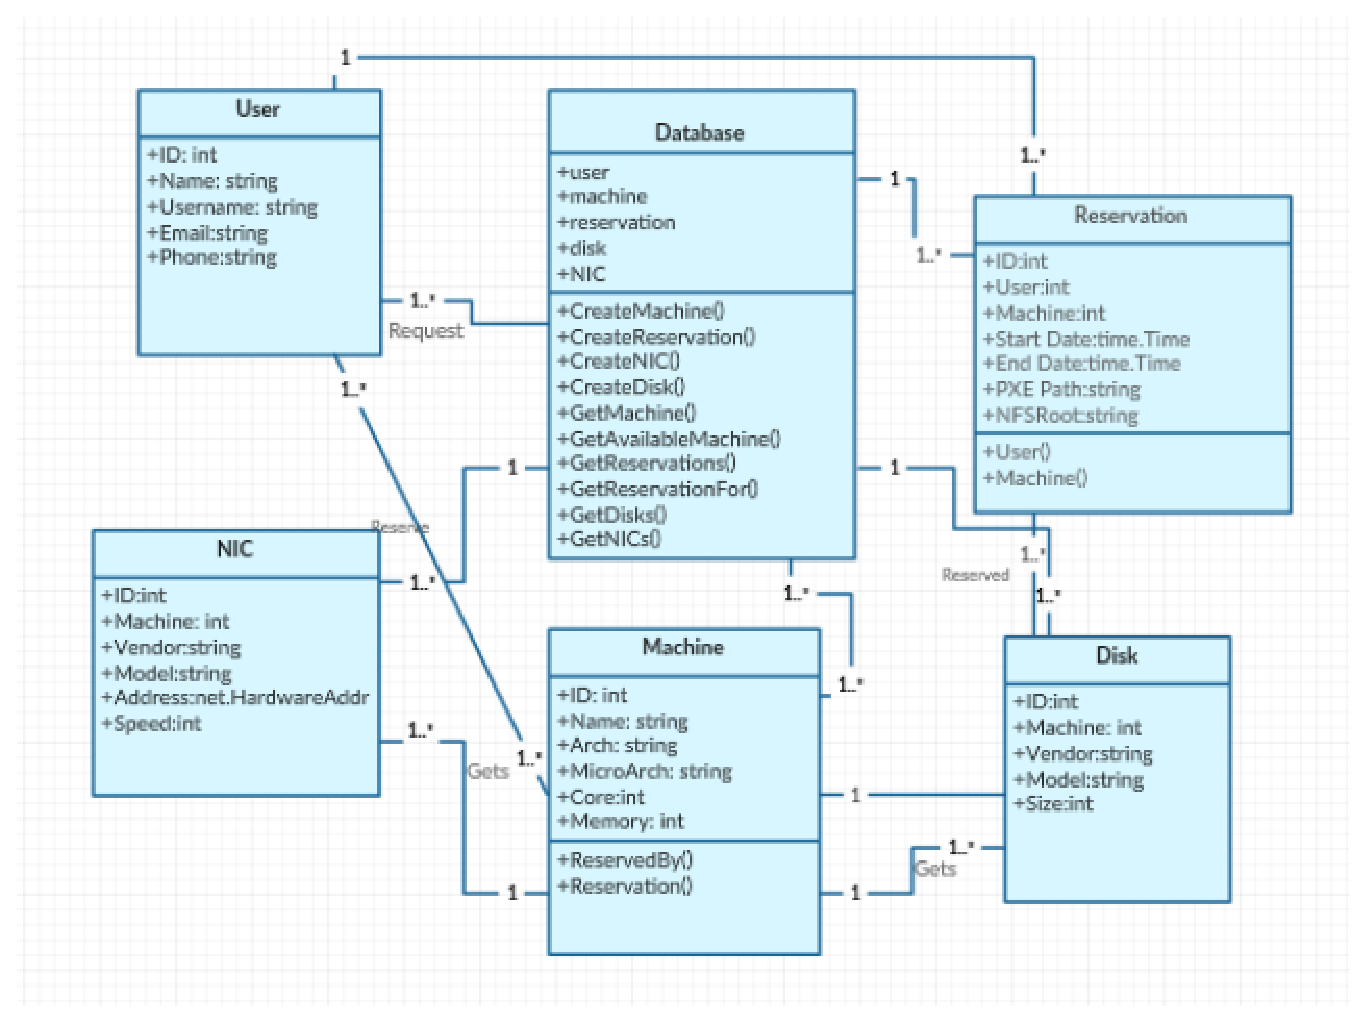
\includegraphics[width = \linewidth]{methods.eps}
\caption{Class Diagram showing struct and method relationships}
\label{sm} 
\end{figure}
\pagebreak
\section{Implementation of Required Functionality}
\section*{Adding Machines to the system}
Adding machines and other devices to the system is one of the software requirements in section \ref{addmachines}. On the user interface, the software provides a text field and forms where users can enter details of machines to be saved as data in the database. The initMachines method creates a new database schema with defined table fields where data is stored. When the user submits a Add Machine form, the data is stored in the table created by initMachines. 
 \autoref{Initializingdatabase} is the code listing for creating the database:
\lstset{basicstyle=\footnotesize\ttfamily,breaklines=true}
\lstset{framextopmargin=50pt,frame=bottomline}
\begin{lstlisting}[caption=Creating table for machines, label=Initializingdatabase]
func initMachines(tx *sql.Tx) error {
	_, err := tx.Exec(`
	CREATE TABLE Machines(
		...........
	);`)
	return err
}
\end{lstlisting}
The CreateMachine method is responsible for inserting data to the database schema. It uses the SQLite INSERT query to parse the given data using the arguments to the database. When the user submits a form (AddMachine), the Go HTTP handler processes this form by converting the plain text to data according to their data types defined in the schema, and then calls CreateMachine to insert this data in the database. \autoref{Addingmachine2} shows the code list.
\begin{lstlisting}[caption=Adding machines details, label=Addingmachine2]
func (d DB) CreateMachine(name string, arch string,
	microarch string, cores int, memoryGB int) error {
	_, err := d.sql.Exec(`
			INSERT INTO Machines(name, arch, microarch,
			 cores, memory)
			VALUES (
				//field values
			)`,
		name, arch, microarch, cores, memoryGB)
	return err
}
\end{lstlisting}

\section*{Making a Reservation}
The reservation process is similar to creating a machine but it requires the User ID and Machine ID as foreign keys in creating a reservation \ref{makereserve}. The User ID is used for selecting the user making the reservation, and Machine ID for selecting the machine to be reserved. On the web interface (reservation page), the form has a drop down list where users can select their user name and the machine they want to reserve. When users open the reservation page to create new reservation, the HTML form use the post request to get list of machines and user name on the drop-down list.

\begin{lstlisting}[caption=Pseudocode, label=addreservation]
\end{lstlisting}
	\begin{enumerate}
	\item Begin transaction.
	\item Select machine and user id from the list where name is chosen and input values.
	\item Check for conflicting input and rollback..
	\item Insert data if conflict doesn't exist.
	\item Commit transaction and return result.
	\end{enumerate}
\begin{lstlisting}[caption=Storing Reservation details, label=Adding reservation]
	 (`BEGIN;
	      	INSERT INTO Reservations (machine,user,start,end,pxepath,nfsroot)
			SELECT (SELECT id from Machines where name=?),(SELECT id from Users where username=?),?,?,?,? where not exists (select r.id from Reservations r 
			INNER JOIN Machines m 
			ON m.id = r.machine where m.name = ? AND (? >= start AND ? <= end) OR (? <= start AND ? >= end));COMMIT;`,machine,user,start,end,pxepath,nfsroot,machine,start,start,end,end)

\end{lstlisting}

To make a reservation, users select their user name and a machine from the drop down list which is loaded by GetMachine and GetUser method. The selection query gets the User ID and the Machine ID of the selected user name and machine as foreign key to the reservation database schema. Also, start and end time/date of the reservation is entered on the text field , and this plain text is formatted to match the database using a time package in Go library. After submitting the form, the Go HTTP handler handles the Insert query by taking all the argument values and saving them to database. 
\subsection*{Concurrency Issues}
Concurrency issue is the condition where two or more threads want to write data into the same storage location in database at same time. It can cause lost of data or affect the integrity of records when one data overrides another entry. In our design, this can occur when there is a conflict between two reservations. Example is when two users want to reserve the same machine with overlapping or same dates. SQLite initiate a transaction for each process to make sure that two processes doesn't access the database in incompatible manner at same time . We implemented a logical condition that checks for data conflict before a reservation process is completed. The logical condition compares the data (date/time) entered with the existing data, and if they conflict or overlaps each other then that reservation process will abort.
\section*{Checking Available Machines}
The user can search the inventory for specific information. One example is the ability to search for available machines in the system as per requirement \ref{searchinventory}. Available machines are those machines that are free for a certain period. This feature helps users to get list of machine free to be reserved. In this process of checking available machines, the user enters a specific start date/time and end date/time in the provided text field, and submits the query. After submiting the query, the HTTP handler processes this request, and the server calls the GetAvailableMachine method of the machine to fetch this request from the database. In this method, we used a SQLite JOIN sub query to combine the machine and reservation database table. It helps to indentify the machines that are not reserved for that time range the user entered. The logic contains SQL WHERE, OR and AND operator to perform comparisons between reservation dates and time. \cite{ANDOR}The AND operator is used to allow multiple conditions in the statement,  the OR operator is used to combine conditions that are true, and the WHERE clause is used to specify condition while fetching data from database\cite{WHEREclause}. 
\autoref{SAM} shows the function and query for this operation.
\begin{lstlisting}[caption=Searching available, label=SAM]
func(d DB) Filter_M_By_Dates(from time.Time, to time.Time) ([]Machine, error){
         rows, err := d.sql.Query(`
		SELECT m.id, name, arch, microarch, cores, memory
		FROM Machines m
		WHERE m.id NOT IN (SELECT r.machine FROM Reservations r
		WHERE (? BETWEEN r.start AND r.end)
		OR (? BETWEEN r.start AND r.end)
		AND  ( r.start BETWEEN ? AND ?) OR (r.end BETWEEN ? AND ?)
	
	); `, from, to, from, to, from, to)
\end{lstlisting}
\section*{Updating Machines details}
As part of the software requirements \ref{addmachines}, users can change the information stored in the database. This is done on the web interface using text box that is attached to every field with that requirement. An example is updating the information of a particular computer or disk when the hardware is upgraded. In this case, the UpdateMachine method performs this action by using the SQLite update query. This update query opens the database schema of the machine and replaces the existing data with a new one.
\autoref{Updatefunction} code listing shows the update function.
\begin{lstlisting}[caption=Function for Updating data, label=Updatefunction]
	_, err := d.sql.Exec(`
			UPDATE Machines
			SET arch = ?, microarch = ?, cores = ?, memory = ?
			WHERE `+row+` = id
	`,arch, microarch, cores, memory)
\end{lstlisting}
\section{Get methods}
The Get methods is used for fetching lists of machines and other devices stored in the database. Each time the user opens the web interface, the HTTP handler sends the server a request and the server calls the GetMachines method to fetch the data from database. This information is listed in the inventory on the web interface through the HTTP Response-Writer. The Get methods use the SQLite selection query to scan through the database and select the required data.  Another usage for Get methods is fetching the details of a machine when the user clicks on a particular machine. A SELECT query and WHERE condition are used in the logic, to specify the machine clicked used its unique ID. This concept is applicable in other struct (type) such as, Disks, NICs and Reservations. 
 
\section{Problems Encountered}
During the implementation, we encountered problems such as parsing plain text to database data types. For example, some functions can parse plain text as they are to the database, but in some cases where the values have a different data type (eg. Hardware Mac address) cant be store as plain text. So this problem was solved by importing functions from the Go library to support those data types. Another issue encountered is trying to combine two database table for search queries. This problem was mostly encountered in the implementation of search query, where two tables were combined for comparing different data.  We solved this query problem by using SQL JOIN function, which normally link different data from multiple database table by scanning through them. With this problem solved, it helped us during the implementation to add more functionality to the user interface without having further error prone situations.



